%short intro
The production of \ZZ in proton-proton collisions has been one of the first di-boson 
processes measured at the LHC. The SM process is and an important and irreducible
background to resonance searches and Higgs production. The production at leading
order is dominated by quark anti-quark annihilation in the $t$ and $u$-channel,
whereas the $s$-channel process is forbidden in the SM 
(see also Figure~\ref{fig:sss-ZZprod-LOdiagrams}). The gluon fusion process 
contributes about 6\% to the total production cross section. 

%FIGURE LO ZZ DIAGRAM
\begin{figure}[htbp]
  \begin{center}
  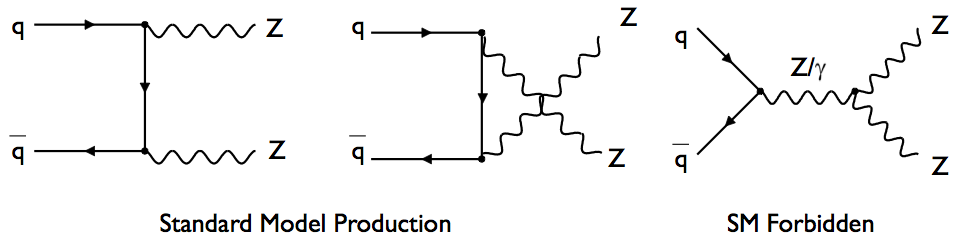
\includegraphics[width=0.9\textwidth]{figures/sss-inclboson-diboson-zzprod-zzdiagram.png}
  \caption{Leading order Feynman diagrams of \ZZ production in the dominant 
  \qqbar\ channel. The \ZZ\ production via the $s$-channel is not allowed in the SM.}
\label{fig:sss-ZZprod-LOdiagrams}
\end{center}
\end{figure}

%decay channels
Precision measurements use the leptonic decay modes of the $Z$ to reduce the impact of
QCD backgrounds. 
The four lepton final state provides an almost background free signature, at the
expense of a relatively small branching ratio 
$BR(ZZ) \to \ll\ll = 0.101^2 \cdot {4 \over 9} = 0.0045$~\cite{PDG}.  
The di-lepton and missing energy channel can exploit the one order of magnitude
higher branching ratio of 
$BR(\ZZ \to \ll\vv) = 0.101 \cdot 0.20 \cdot 2 \cdot {2 \over 3} = 0.0269$, 

%analysis CMS and ATLAS.
%ATLAS ZZ 7 TeV~\cite{Aad:2012awa}
%CMS ZZ4l 8 TeV~\cite{Khachatryan:2014dia}
%CMS ZZ4l 7 TeV~\cite{Chatrchyan:2012sga}
%CMS ZZ2l2nu 7+8 TeV~\cite{Khachatryan:2015pba}
The ATLAS collaboration has published results on the $7\TeV$ data-set 
in the $\ll\ll$ and $\ll\vv$ final state~\cite{Aad:2012awa}. The CMS collaboration
has analysed the full 7 and $8\TeV$ data sets in both 
the $\ll\ll$~\cite{Chatrchyan:2012sga,Khachatryan:2014dia} and 
$\ll\vv$ final state~\cite{Khachatryan:2015pba}.

%Theoretical calculations
% NLO alpha_s arXiv:1105.0020
% NLO alpha_EKW arXiv:1305.5402,arXiv:1307.4331
Theoretical predictions for $\ZZ$ production are available 
at NLO in $\alpha_s$~\cite{arXiv:1105.0020}. In addition, electroweak 
corrections at NLO have been calculated~\cite{arXiv:1305.5402,arXiv:1307.4331}. 

%Selections
The event selection for the $\ll\ll$ final state requires exactly four leptons 
fulfilling a set of cuts on kinematic quantities. ATLAS and CMS use similar criteria 
as listed in detail in Table~\ref{tab:sss-ZZprod-cuts}. While ATLAS uses $l=e,\mu$,
CMS includes also $\Z\to\tautau$ with subsequent hadronic and leptonic $\tau$
decays. ATLAS uses in addition forward leptons outside the ID tracker
to increase the acceptance by 6\% for electrons and 10\% for muons.

%Backgrounds

% Results at the end?
Besides the total cross section for the $pp \to \ZZ$ production process, both
experiments measure also fiducial and differential cross sections, and provide
limits on anomalous neutral triple gauge boson couplings.




